\documentclass[a4paper, 14pt]{extarticle}
\usepackage[russian]{babel}
\usepackage[T1]{fontenc}
\usepackage{fontspec}
\usepackage{indentfirst}
\usepackage{enumitem}
\usepackage{graphicx}
\usepackage[
  left=20mm,
  right=10mm,
  top=20mm,
  bottom=20mm
]{geometry}
\usepackage{parskip}
\usepackage{titlesec}
\usepackage{xurl}
\usepackage{hyperref}
\usepackage{float}
\usepackage[
  figurename=Рисунок,
  labelsep=endash,
]{caption}
\usepackage[outputdir=build, newfloat]{minted}

\hypersetup{
  colorlinks=true,
  linkcolor=black,
  filecolor=blue,
  urlcolor=blue,
}

\renewcommand*{\labelitemi}{---}
\setmainfont{Times New Roman}
\setmonofont{JetBrains Mono}[
  SizeFeatures={Size=11},
]

\newenvironment{code}{\captionsetup{type=listing}}{}
\SetupFloatingEnvironment{listing}{name=Листинг}

\setminted[python]{
  fontsize=\footnotesize,
  frame=lines,
  framesep=2mm,
}

\setlength{\parskip}{6pt}

\setlength{\parindent}{1cm}
\setlist[itemize]{itemsep=0em,topsep=0em,parsep=0em,partopsep=0em,leftmargin=2.0cm,wide}
\setlist[enumerate]{itemsep=0em,topsep=0em,parsep=0em,partopsep=0em,leftmargin=2.0cm,wide}

\renewcommand{\thesection}{\arabic{section}.}
\renewcommand{\thesubsection}{\thesection\arabic{subsection}.}
\renewcommand{\thesubsubsection}{\thesubsection\arabic{subsubsection}.}

\titleformat{\section}{\normalfont\bfseries}{\thesection}{0.5em}{}
\titleformat{\subsection}{\normalfont\bfseries}{\thesubsection}{0.5em}{}

\titleformat*{\section}{\normalfont\bfseries}
\titleformat*{\subsection}{\normalfont\bfseries}

\linespread{1.5}
\renewcommand{\baselinestretch}{1.5}

\begin{document}

\begin{titlepage}
  \vspace{0pt plus2fill}
  \noindent

  \vspace{0pt plus6fill}
  \begin{center}
    Санкт-Петербургский национальный исследовательский университет
    информационных технологий, механики и оптики

    \vspace{0pt plus3fill}

    Факультет инфокоммуникационных технологий

    Направление подготовки 11.03.02

    \vspace{0pt plus2fill}

    \textbf{ПРАКТИЧЕСКАЯ РАБОТА}

  \end{center}

  \vspace{0pt plus9fill}
  \begin{flushright}
    Выполнил: \\
    Швалов Даниил Андреевич

    Группа: К33211

    Проверил: \\
    Меркушев Александр Евгеньевич
  \end{flushright}

  \vspace{0pt plus2fill}
  \begin{center}
    Санкт-Петербург

    2023
  \end{center}
\end{titlepage}

\setcounter{page}{2}

\section*{Упражнение 1}

В данном упражнении необходимо установить и настроить среду для работы с
mininet. В качестве рабочей машины я использую MacBook с процессором M1. В связи
с этим у меня возникли проблемы с установкой и использованием виртуальной
машины. Поэтому для работы с mininet была использована выделенная виртуальная
машина RUVDS (рис. \ref{fig:ruvds})

\begin{figure}[H]
  \centering
  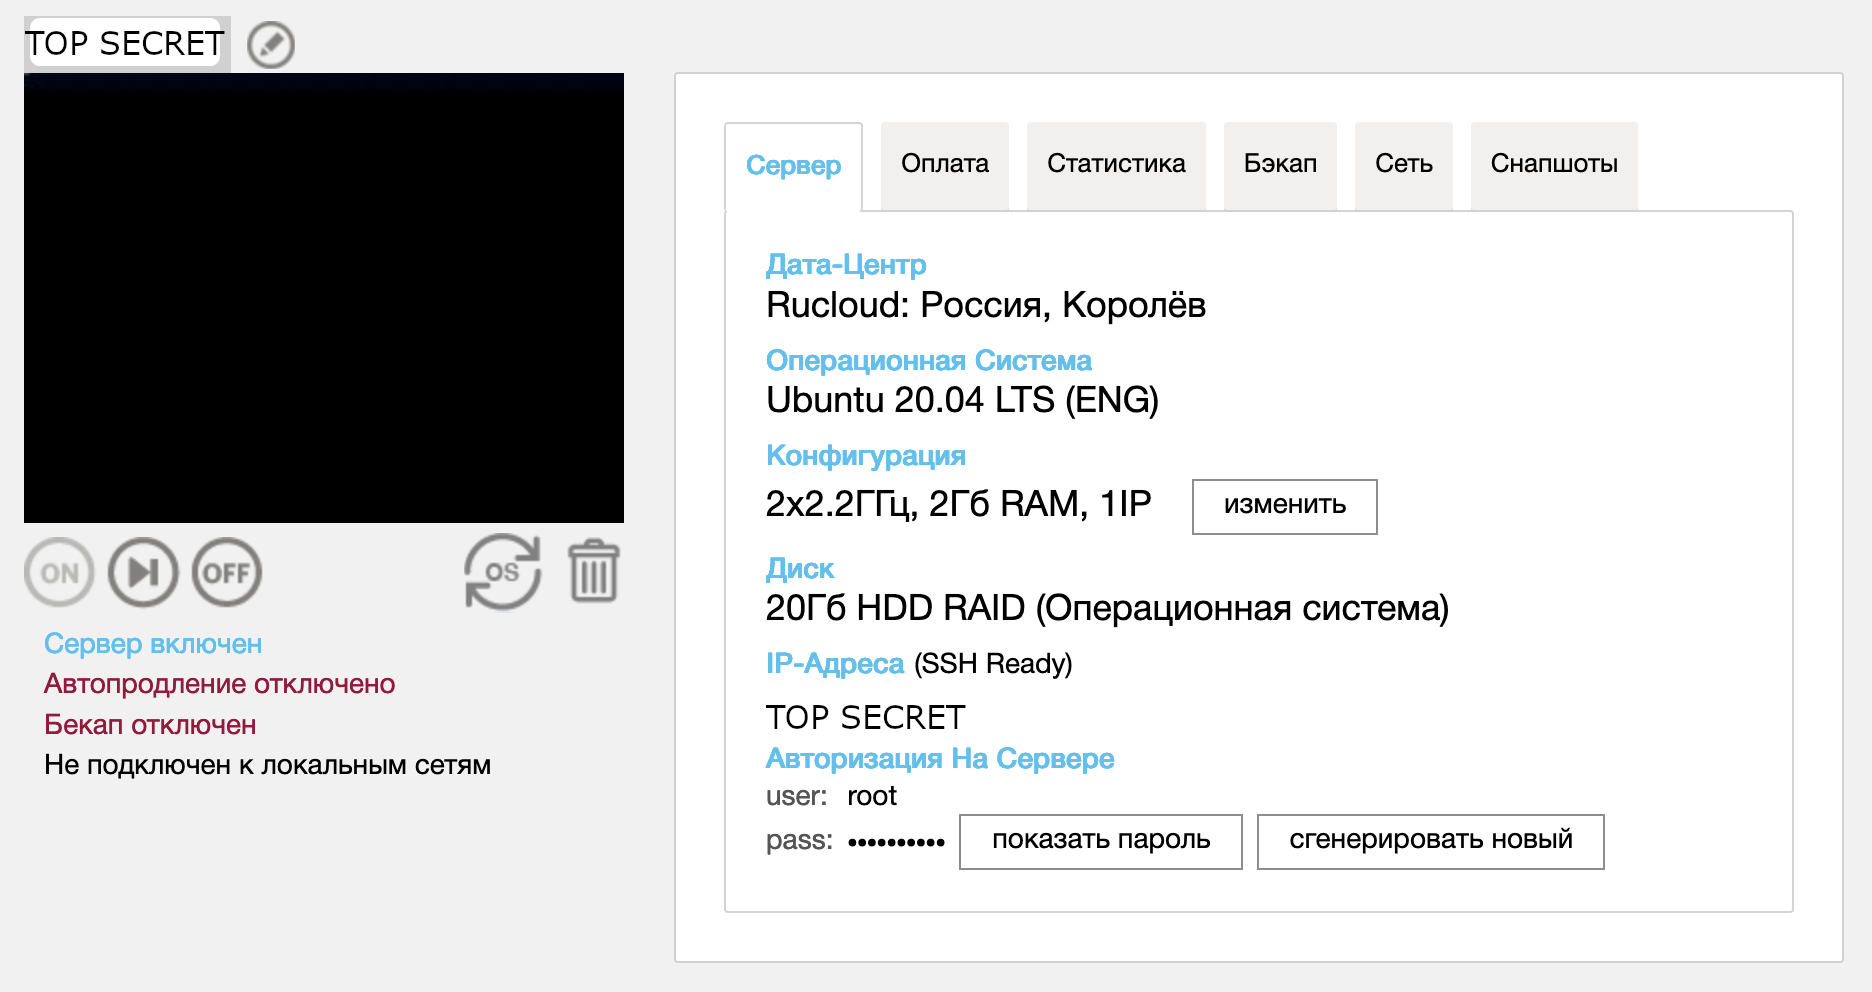
\includegraphics[width=\textwidth]{images/ruvds.png}
  \caption{Виртуальная машина RUVDS}
  \label{fig:ruvds}
\end{figure}

Вследствие этого, mininet был установлен в систему нативно. Для этого я проделал
следующие шаги:
\begin{enumerate}
  \item склонировал исходный код mininet с помощью команды
  \begin{minted}{text}
       git clone https://github.com/mininet/mininet
  \end{minted}
  \item выбрал последнюю стабильную версию mininet с помощью команд
  \begin{minted}{text}
       cd mininet
       git tag  # list available versions
       git checkout -b mininet-2.3.0 2.3.0
       cd ..
  \end{minted}
  \item установил mininet в систему с помощью команды
  \begin{minted}{text}
       mininet/util/install.sh -a
  \end{minted}
\end{enumerate}

После этого mininet был успешно установлен на мою виртуальную машину (рис.
\ref{fig:mininet}).

\begin{figure}[H]
  \centering
  \fbox{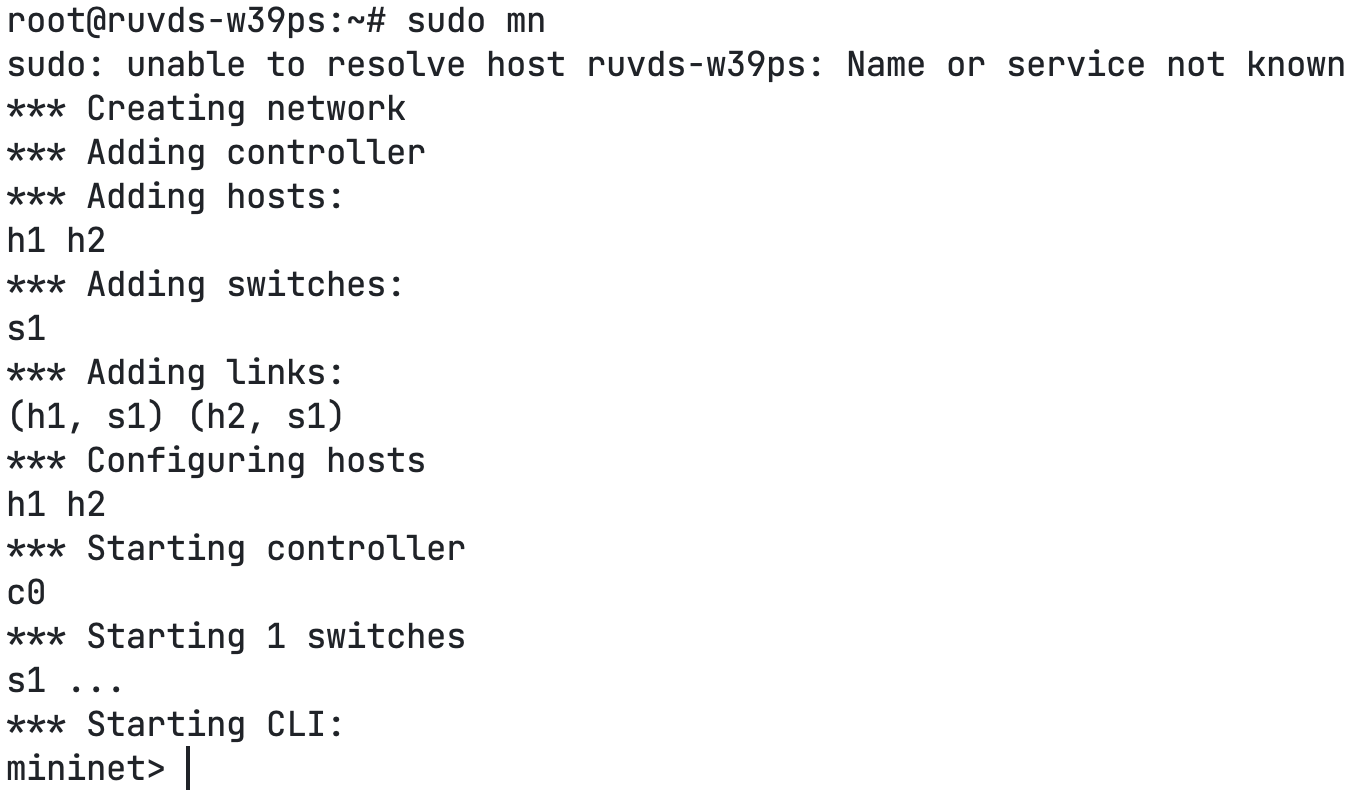
\includegraphics[width=0.9\textwidth]{images/mininet.png}}
  \caption{Проверка работоспособности mininet}
  \label{fig:mininet}
\end{figure}

\section*{Упражнение 2}

В этом упражнении необходимо создать собственную топологию с использованием
API-интерфейса mininet на языке python. В начале необходимо было создать
линейную топологию, изображенную на рис. \ref{fig:linear-topology}.

\begin{figure}[H]
  \centering
  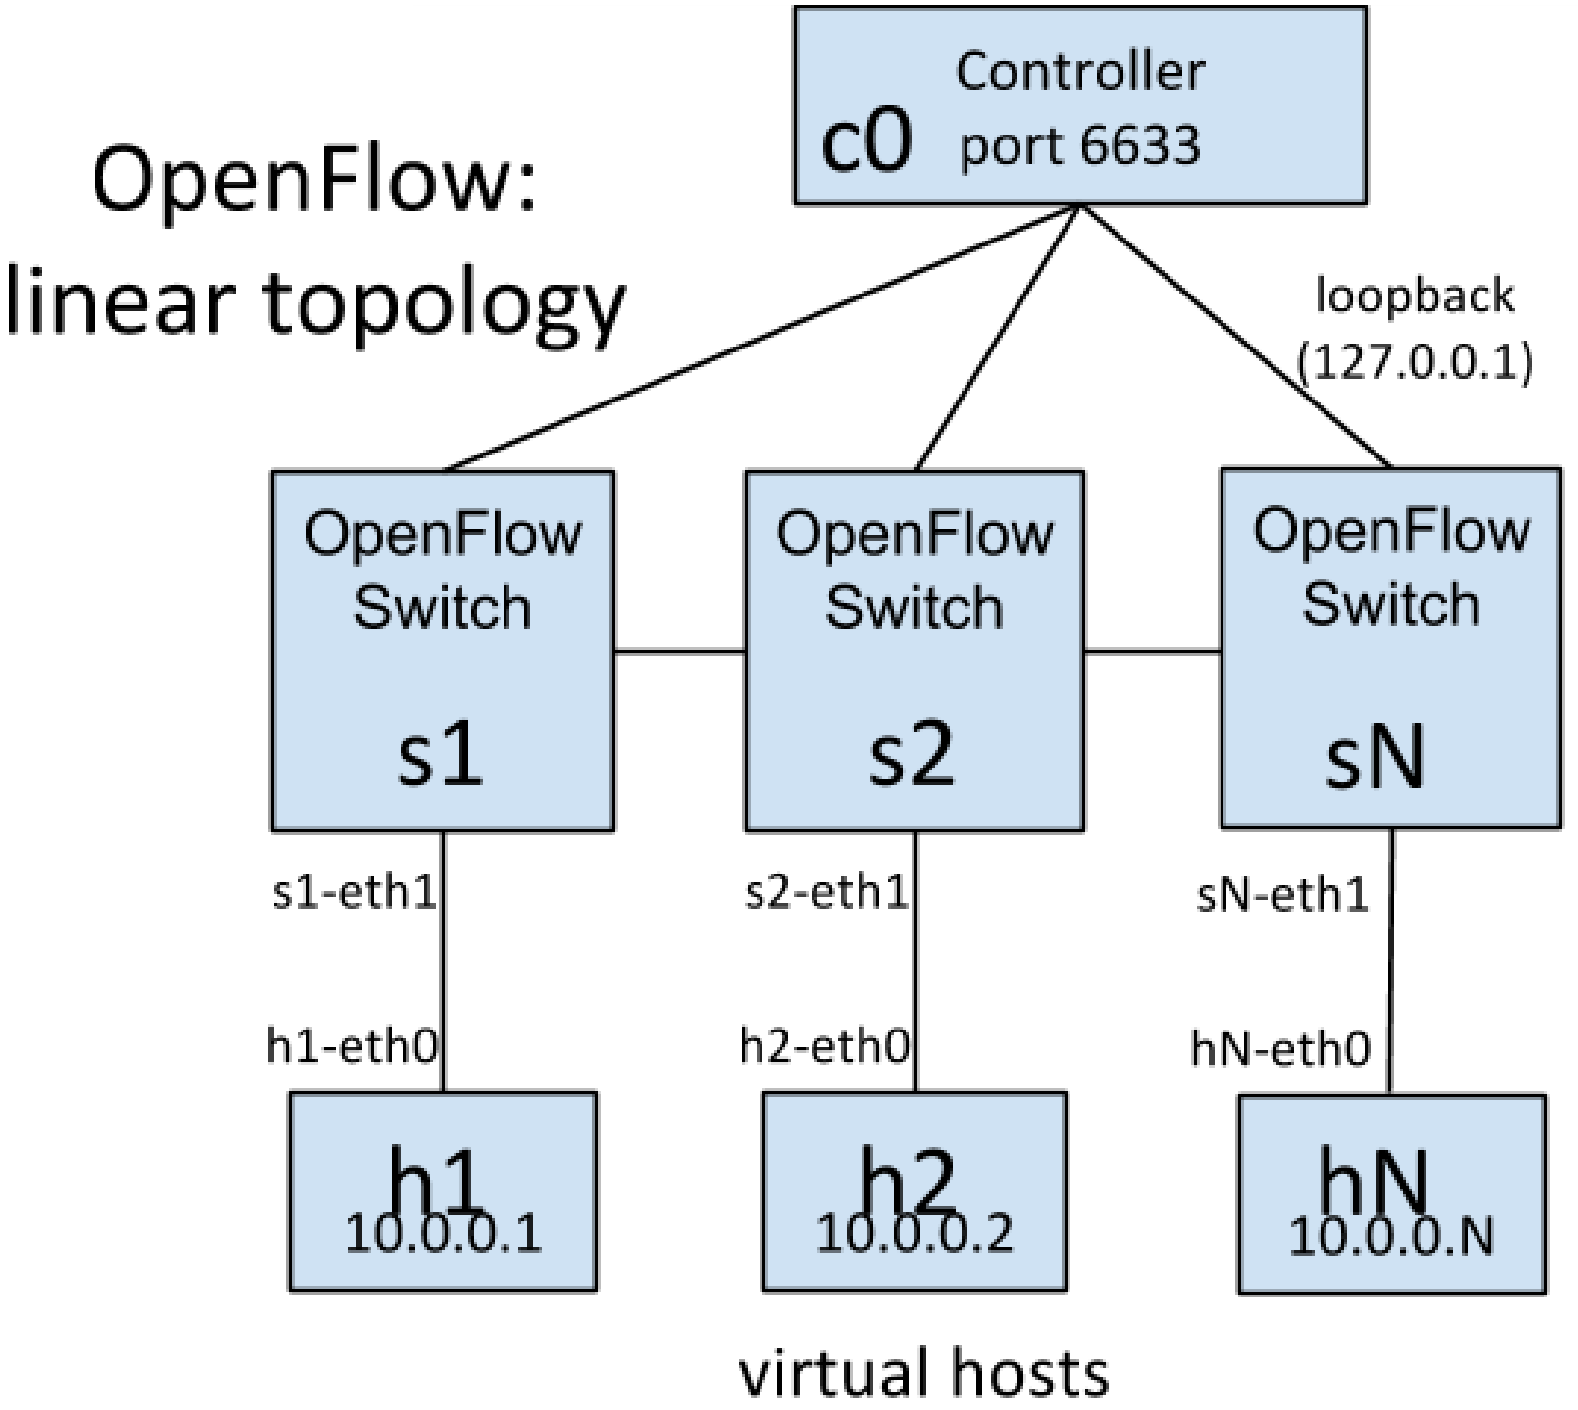
\includegraphics[width=0.7\textwidth]{images/linear-topology.png}
  \caption{Схема линейной топологии}
  \label{fig:linear-topology}
\end{figure}

Исходный код скрипта, реализующего линейную топологию, находится в приложении
\ref{app:LinearTopo.py}. На рис. \ref{fig:linear-py} изображен результат запуска
скрипта.

\begin{figure}[H]
  \centering
  \fbox{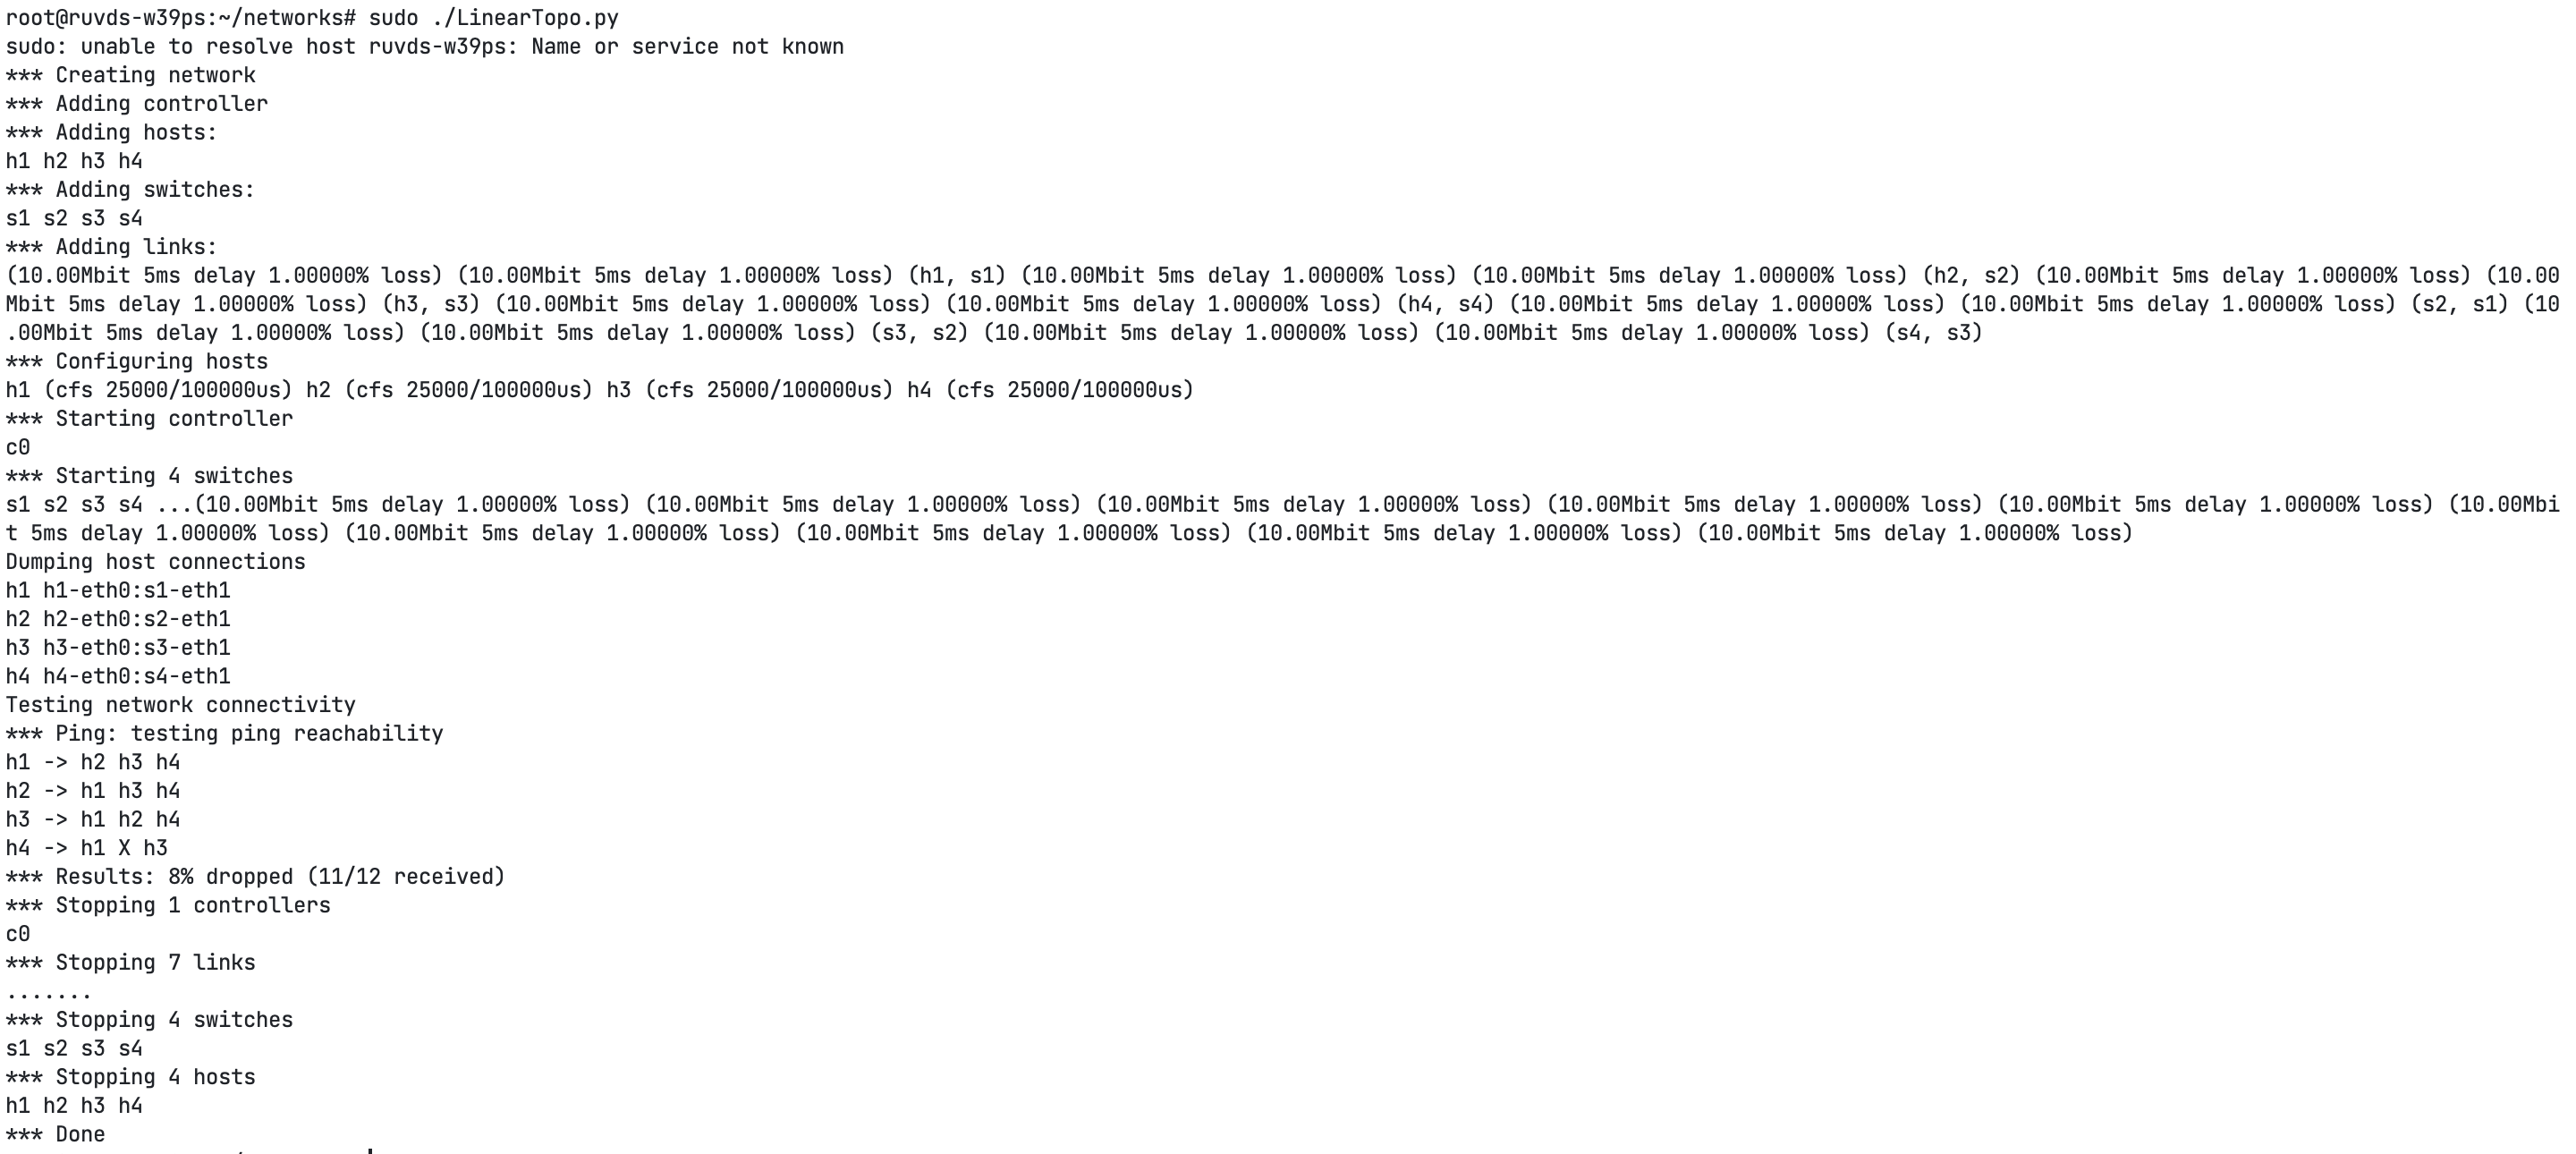
\includegraphics[width=\textwidth]{images/linear-py.png}}
  \caption{Результат запуска скрипта линейной топологии}
  \label{fig:linear-py}
\end{figure}

В следующем задании было необходимо создать простую топологию дерева,
изображенную на рис. \ref{fig:tree-topology}.

\begin{figure}[H]
  \centering
  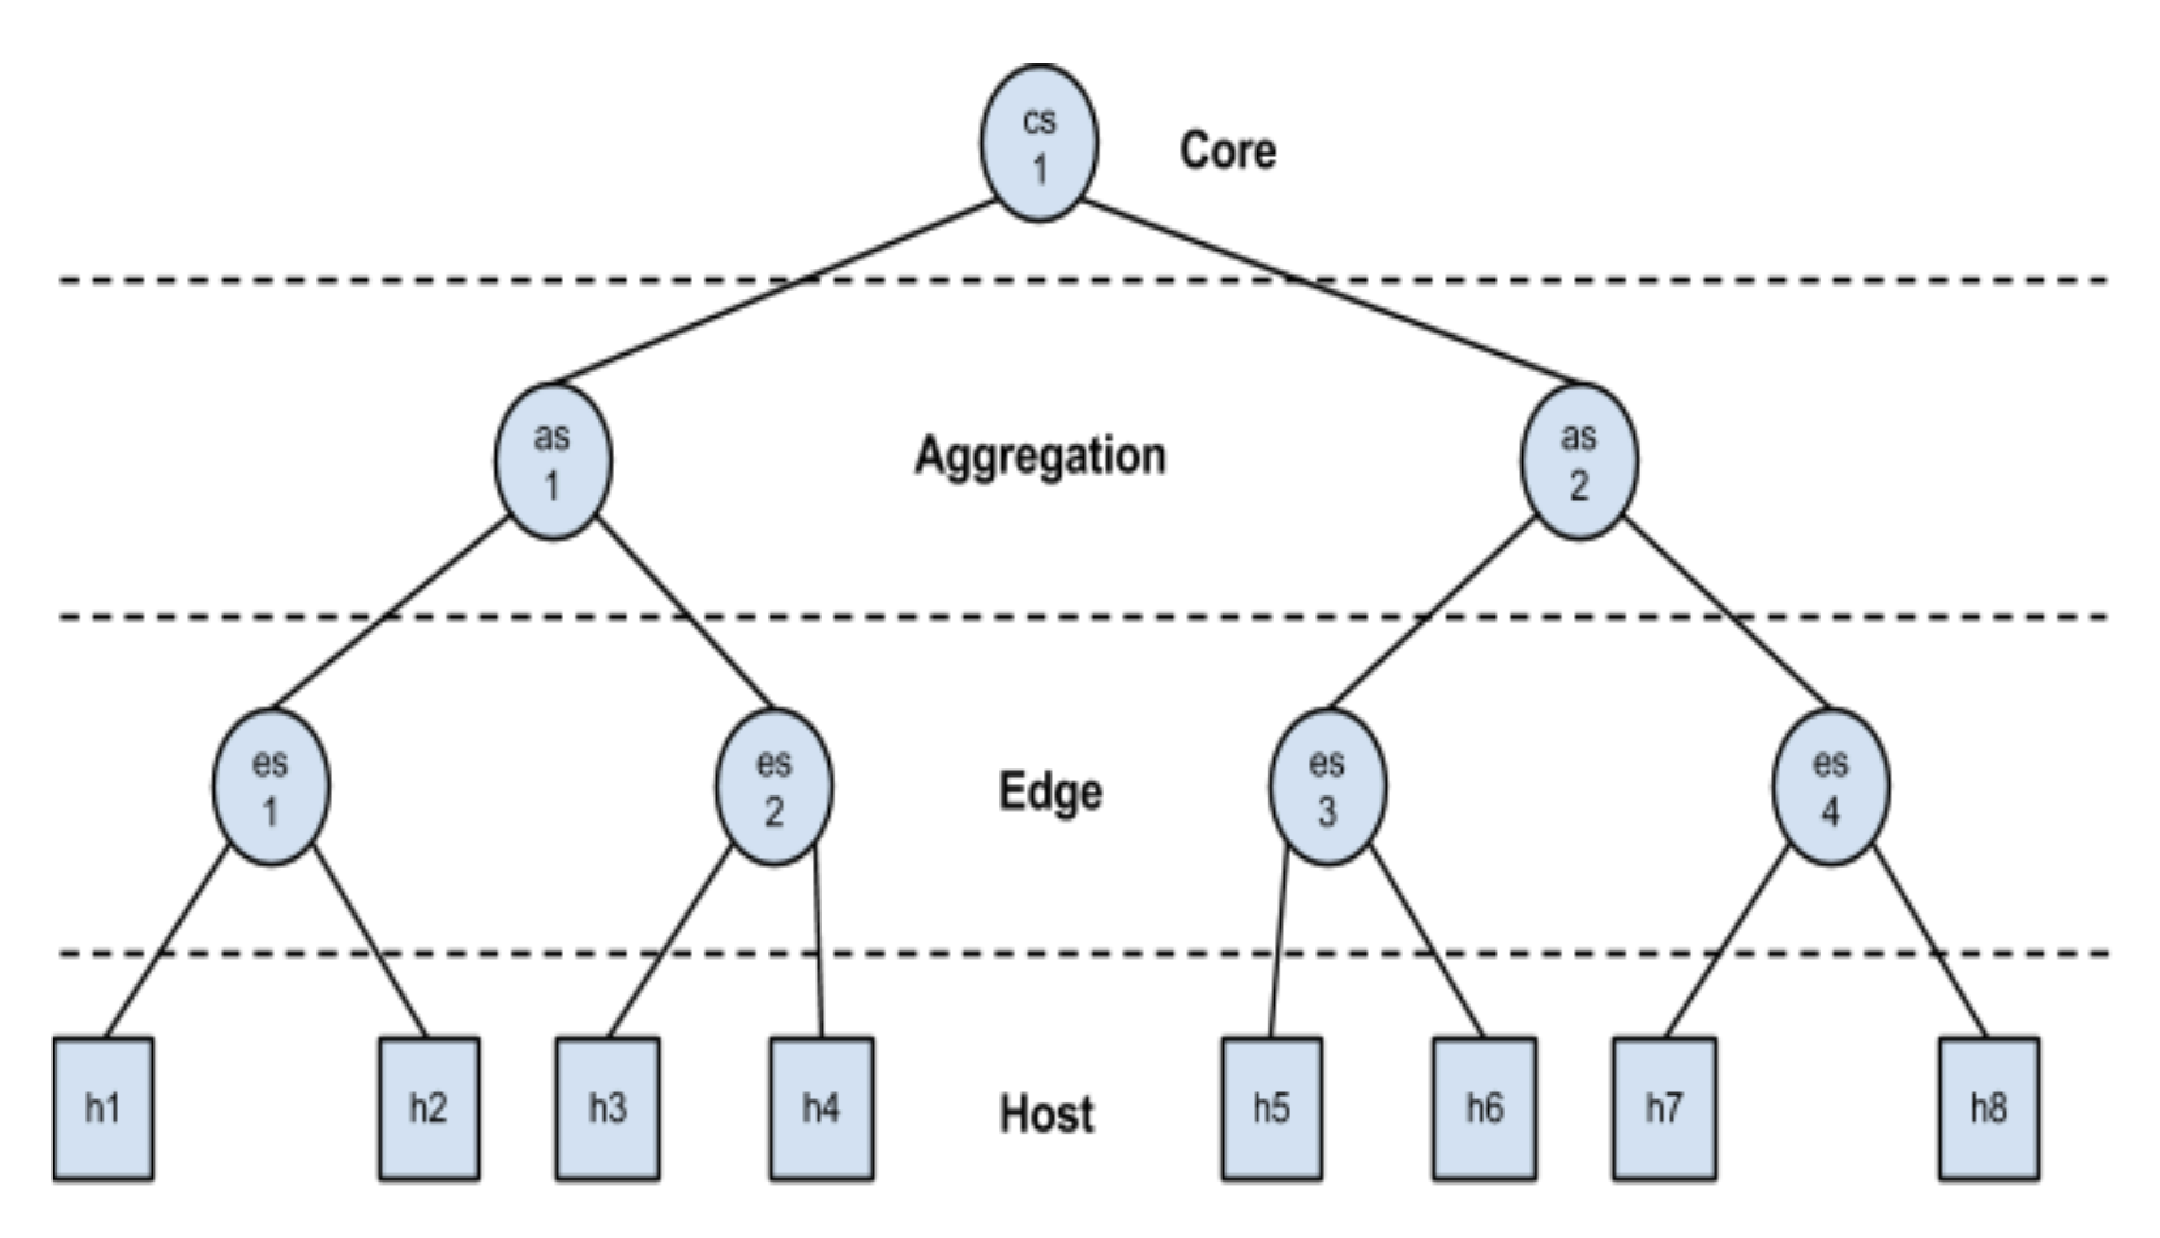
\includegraphics[width=0.9\textwidth]{images/tree-topology.png}
  \caption{Схема древовидной топологии с разветвлением равным 2}
  \label{fig:tree-topology}
\end{figure}

Исходный код скрипта, реализующего древовидную топологию, находится в приложении
\ref{app:CustomTopo.py}. На рис. \ref{fig:tree-py} изображен результат запуска
скрипта.

\begin{figure}[H]
  \centering
  \fbox{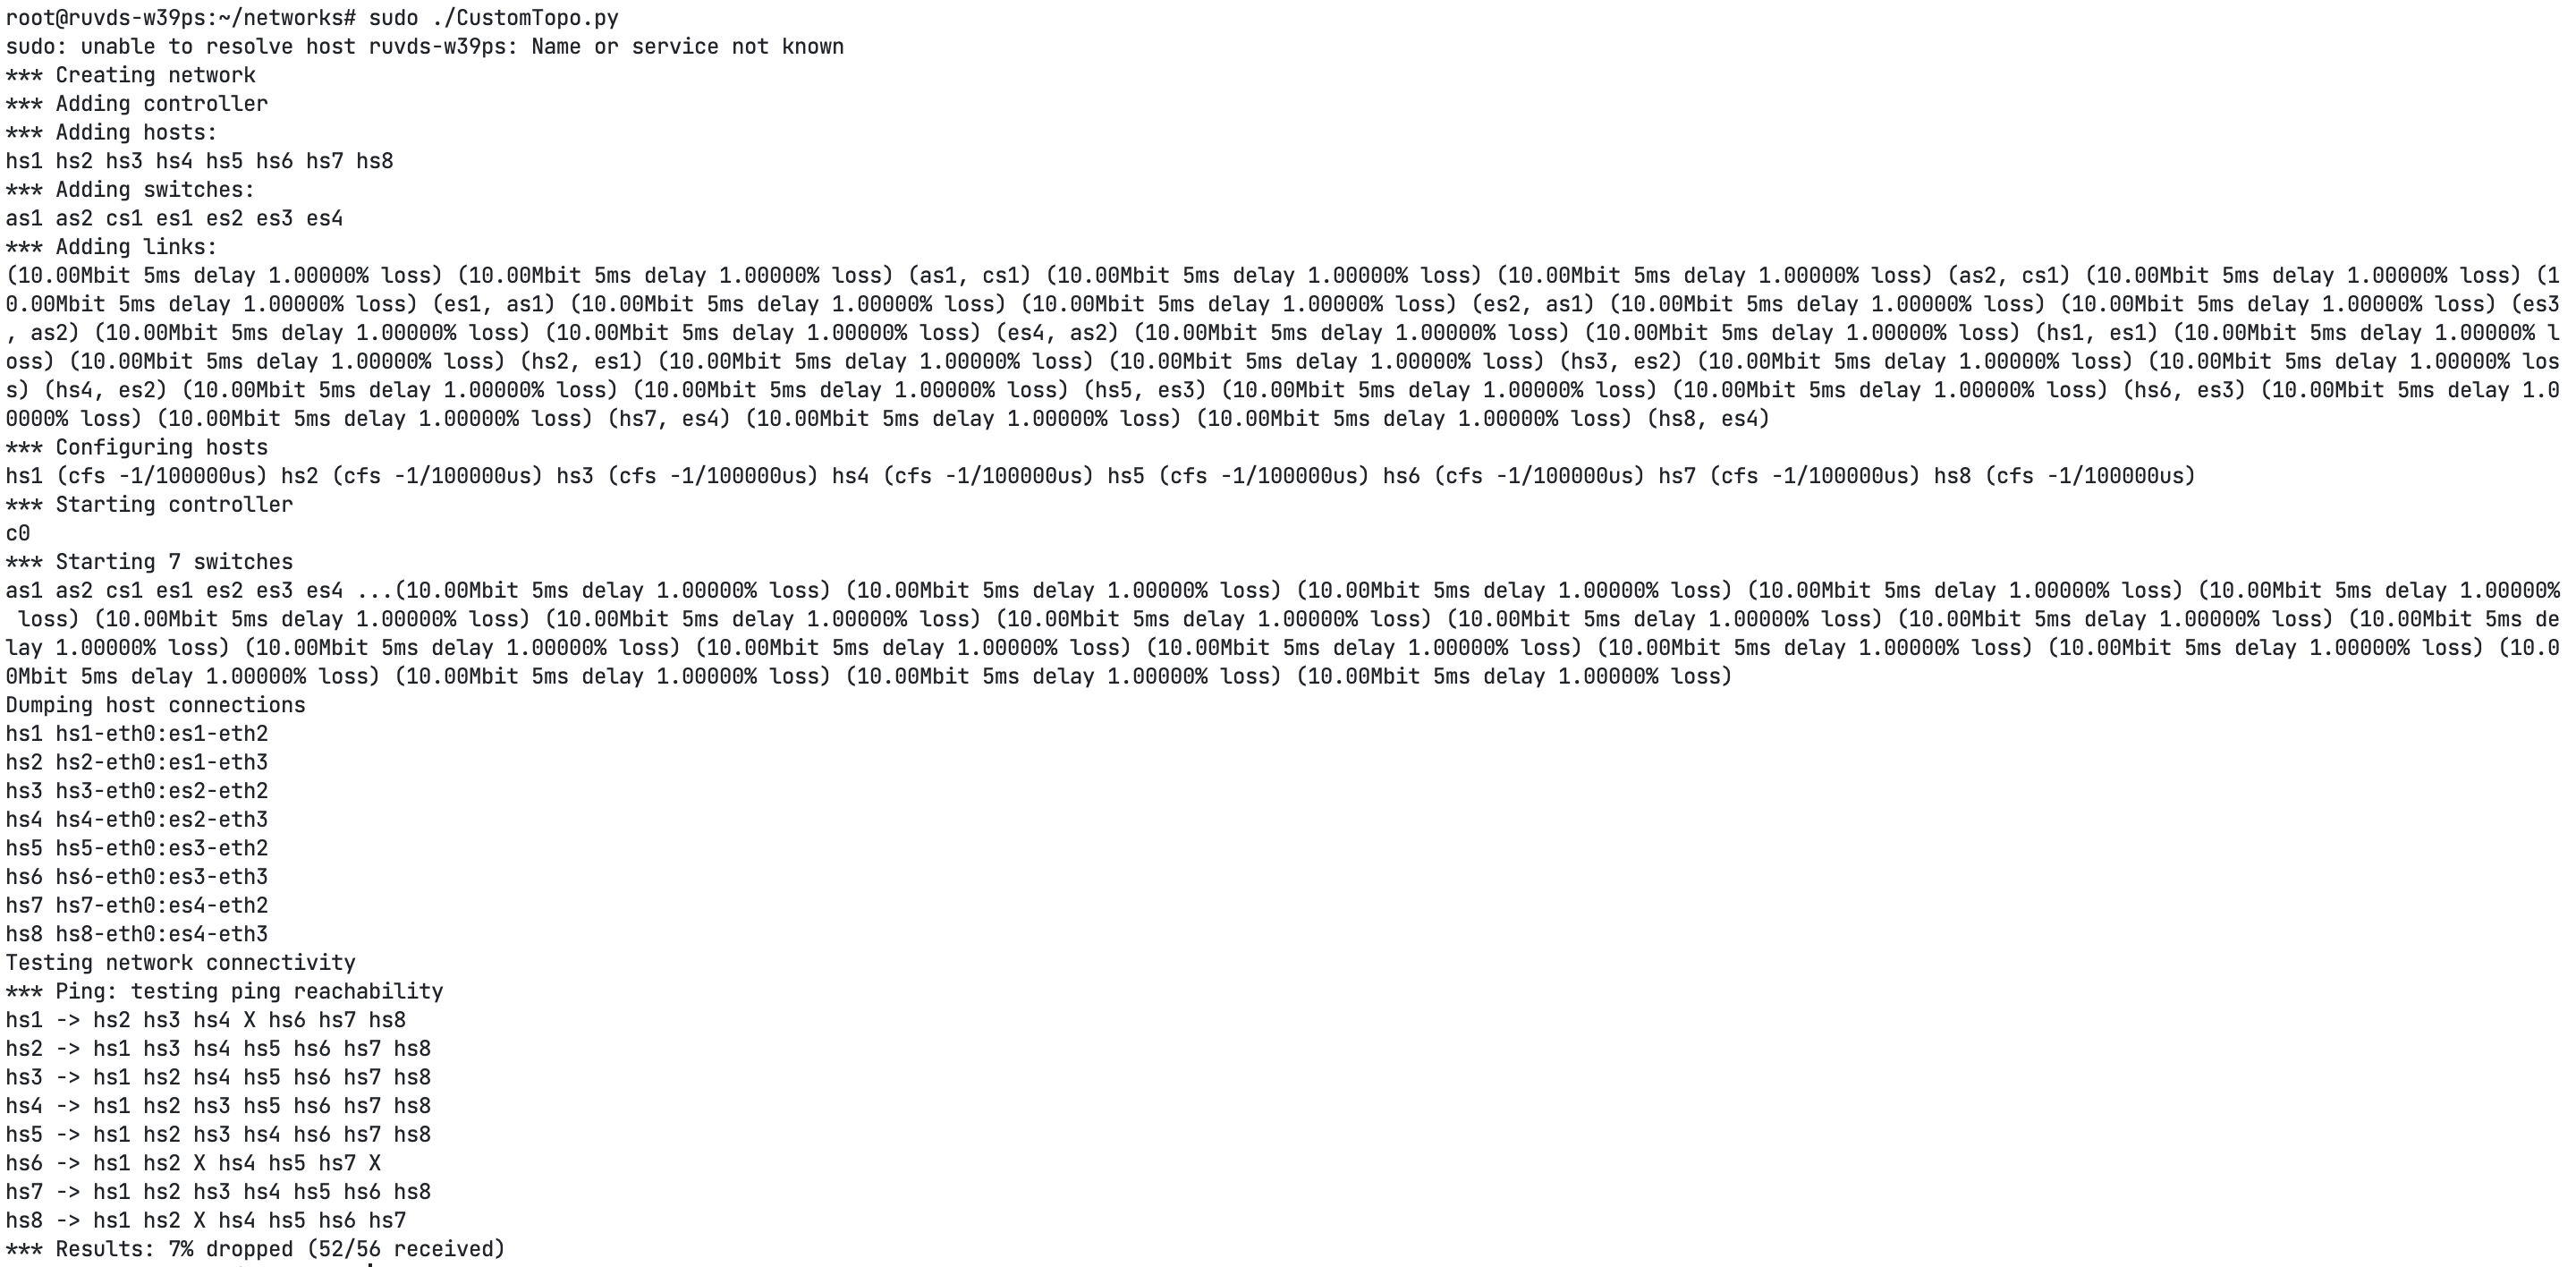
\includegraphics[width=\textwidth]{images/tree-py.png}}
  \caption{Результат запуска скрипта древовидной топологии}
  \label{fig:tree-py}
\end{figure}

\section*{Упражнение 3}

В данном упражнении необходимо использовать POX и протестировать доступность
хостов. В начале был выключен предыдущий контроллер и очищен mininet (рис.
\ref{fig:mininet-cleanup}).

\begin{figure}[H]
  \centering
  \fbox{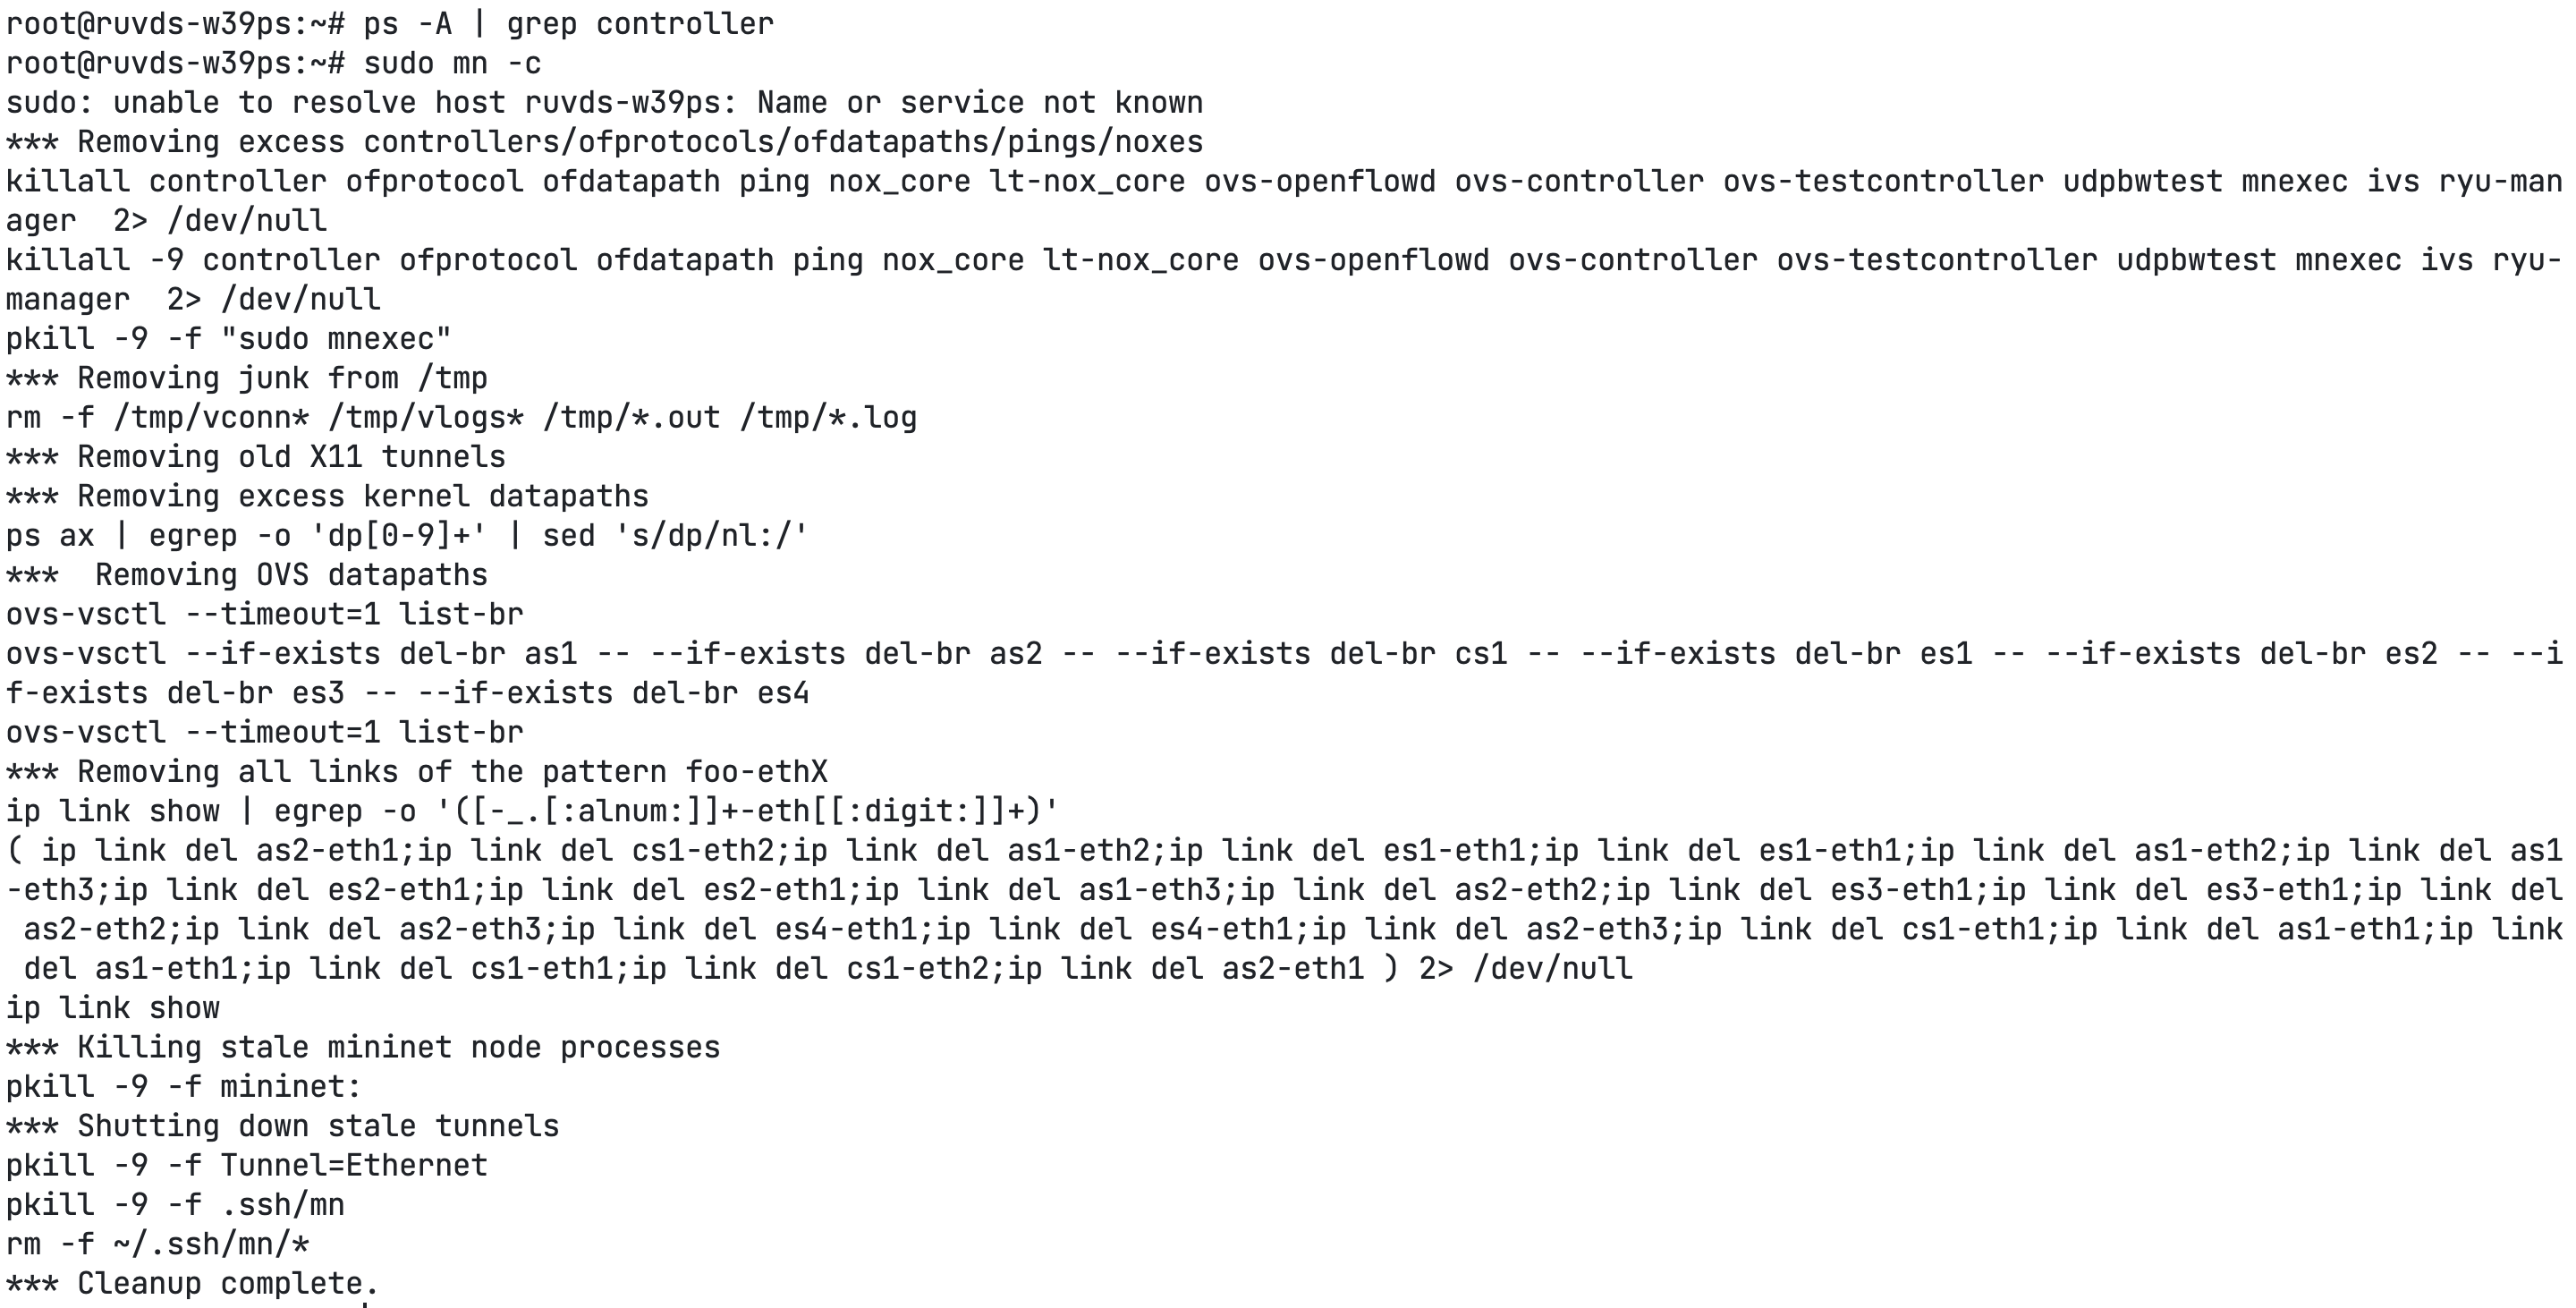
\includegraphics[width=0.9\textwidth]{images/mininet-cleanup.png}}
  \caption{Отключение предыдущего контроллера и очистка mininet}
  \label{fig:mininet-cleanup}
\end{figure}

После этого был запущен POX (рис. \ref{fig:pox}) и mininet (рис.
\ref{fig:mininet-start}).

\begin{figure}[H]
  \centering
  \fbox{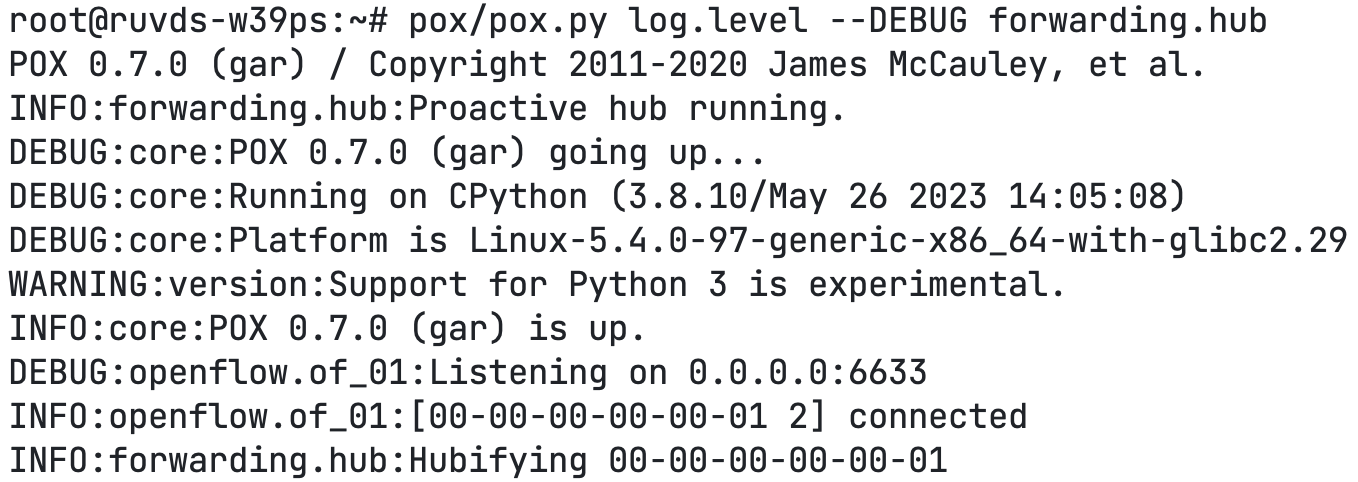
\includegraphics[width=0.7\textwidth]{images/pox.png}}
  \caption{Запуск POX}
  \label{fig:pox}
\end{figure}

\begin{figure}[H]
  \centering
  \fbox{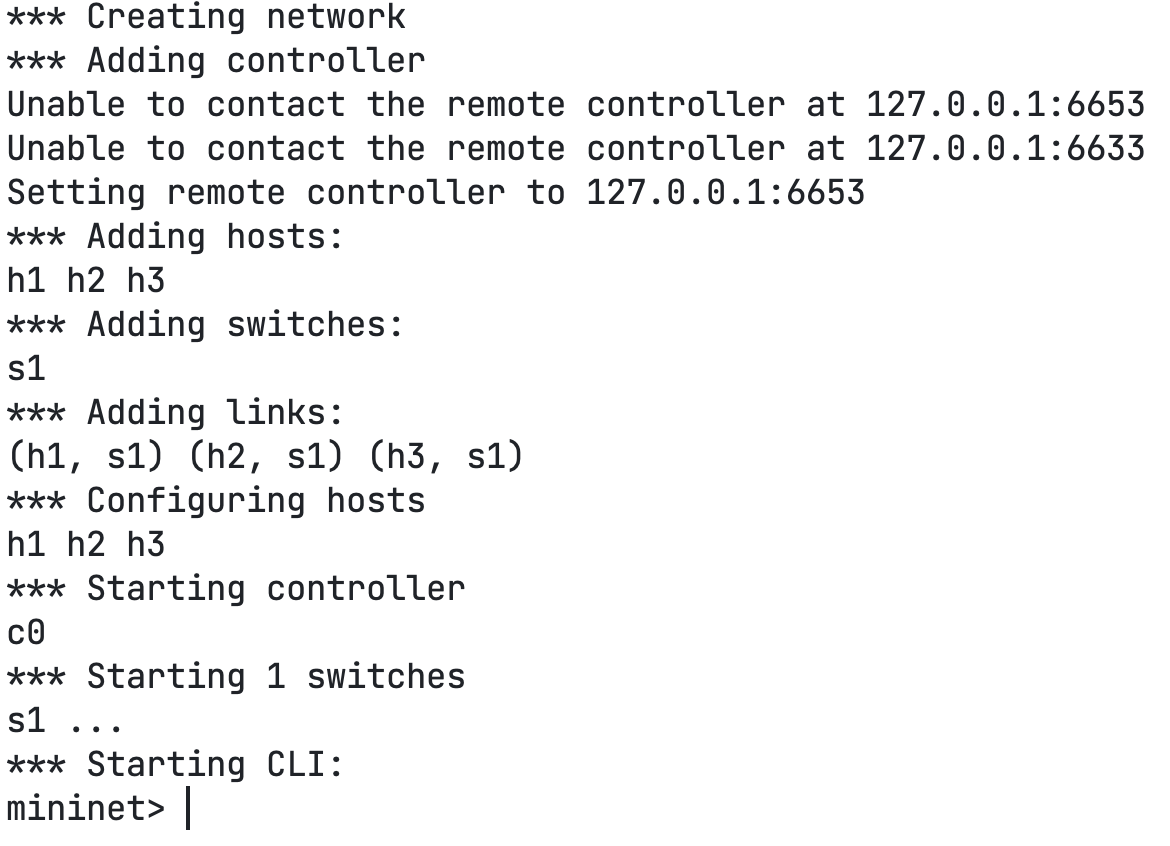
\includegraphics[width=0.7\textwidth]{images/mininet-start.png}}
  \caption{Запуск mininet}
  \label{fig:mininet-start}
\end{figure}

Затем в терминале mininet была выполнена команда \texttt{xterm h1 h2 h3},
которая создала три терминала. Во втором терминале была выполнена команда
\texttt{tcpdump -XX -n -i h2-eth0}, а в третьем --- команда \texttt{tcpdump -XX
  -n -i h3-eth0}. Тем самым был запущен tcpdump для второго и третьего хостов
для печати пакетов, просматриваемых хостом. В первом терминале была выполнена
команда \texttt{ping -c1 10.0.0.2}, которая проверяет доступность хоста с
адресом 10.0.0.2 (рис. \ref{fig:ping-exists}). На рис. \ref{fig:arp-exists}
изображено то, что вывел tcpdump после ping-запроса. Как видно, данный хост
существует и доступен.

\begin{figure}[H]
  \centering
  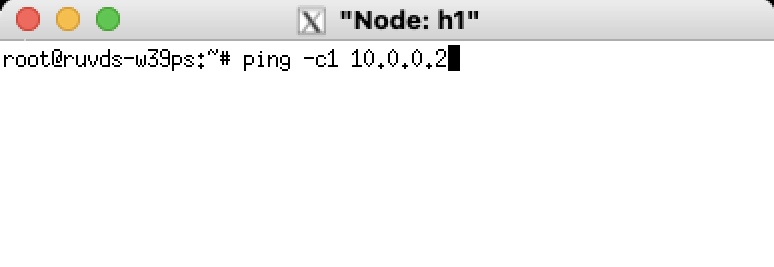
\includegraphics[width=0.7\textwidth]{images/ping-exists.png}
  \caption{Проверка доступности хоста с адресом 10.0.0.2}
  \label{fig:ping-exists}
\end{figure}

\begin{figure}[H]
  \centering
  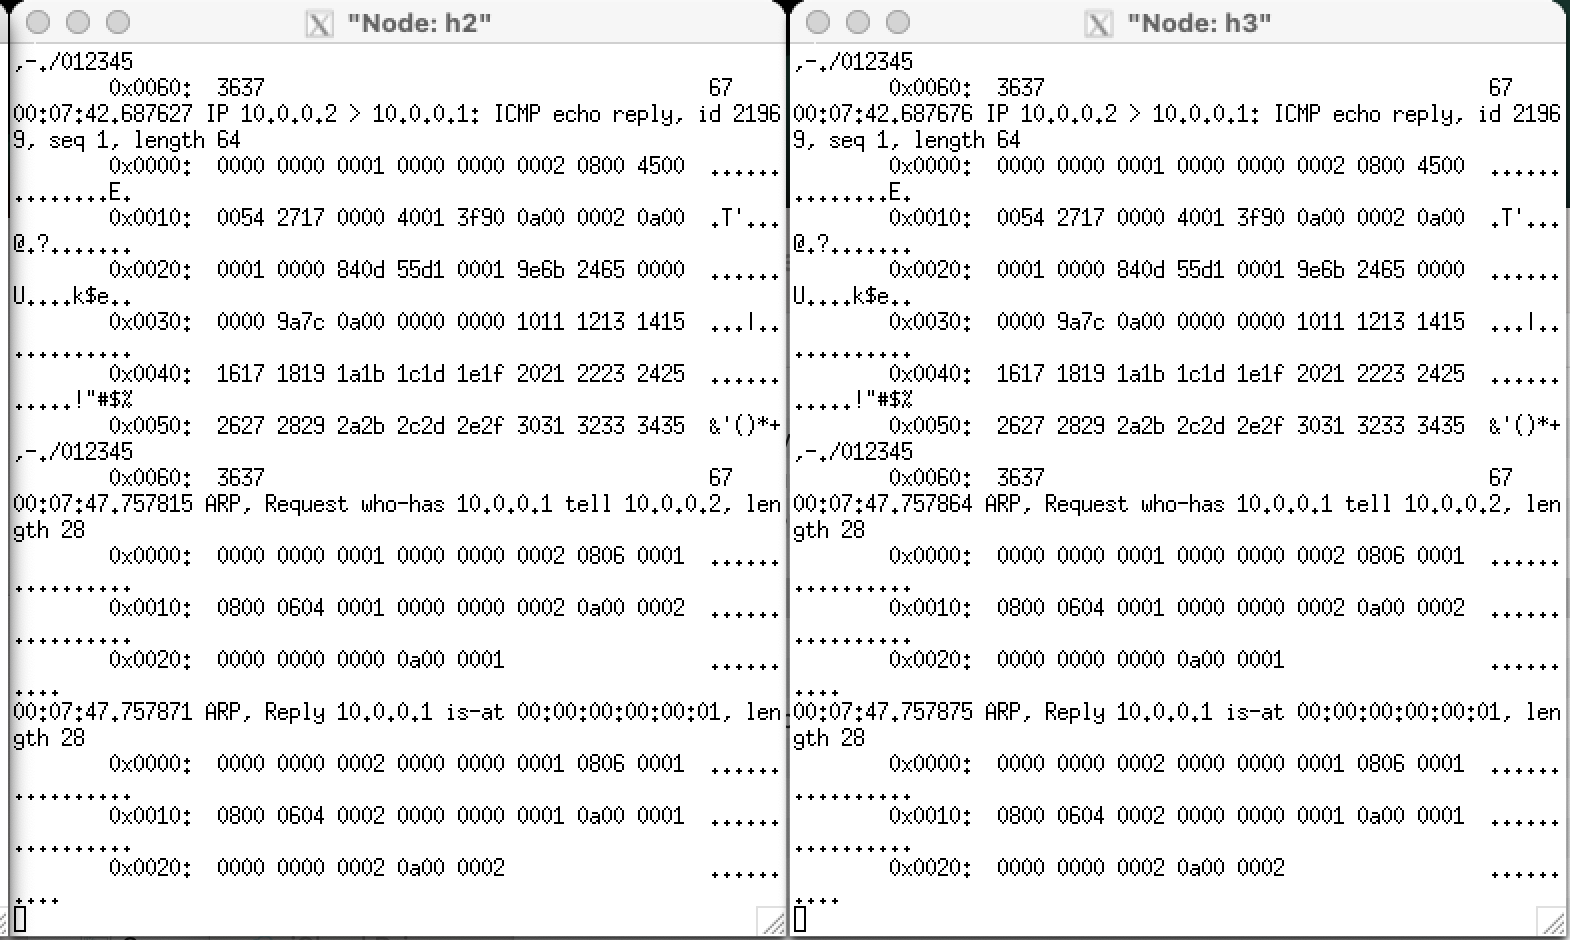
\includegraphics[width=\textwidth]{images/arp-exists.png}
  \caption{Вывод tcpdump после первого запроса ping}
  \label{fig:arp-exists}
\end{figure}

В случае, если проверить доступность несуществующего хоста с адресом 10.0.0.5
(рис. \ref{fig:ping-non-exists}), то в выводе tcpdump будет видно, что хост не
был найден (рис. \ref{fig:arp-non-exists}).

\begin{figure}[H]
  \centering
  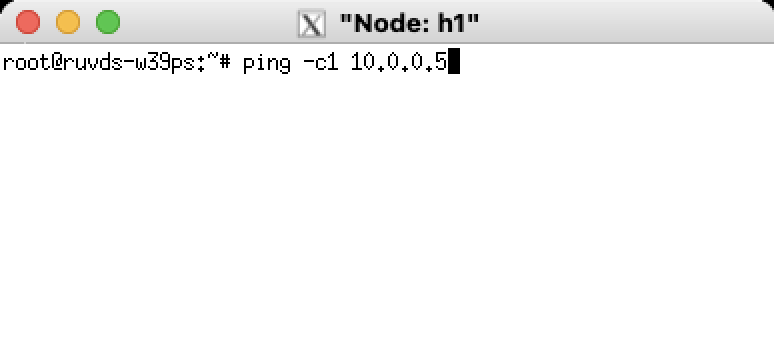
\includegraphics[width=0.7\textwidth]{images/ping-non-exists.png}
  \caption{Проверка доступности хоста с адресом 10.0.0.5}
  \label{fig:ping-non-exists}
\end{figure}

\begin{figure}[H]
  \centering
  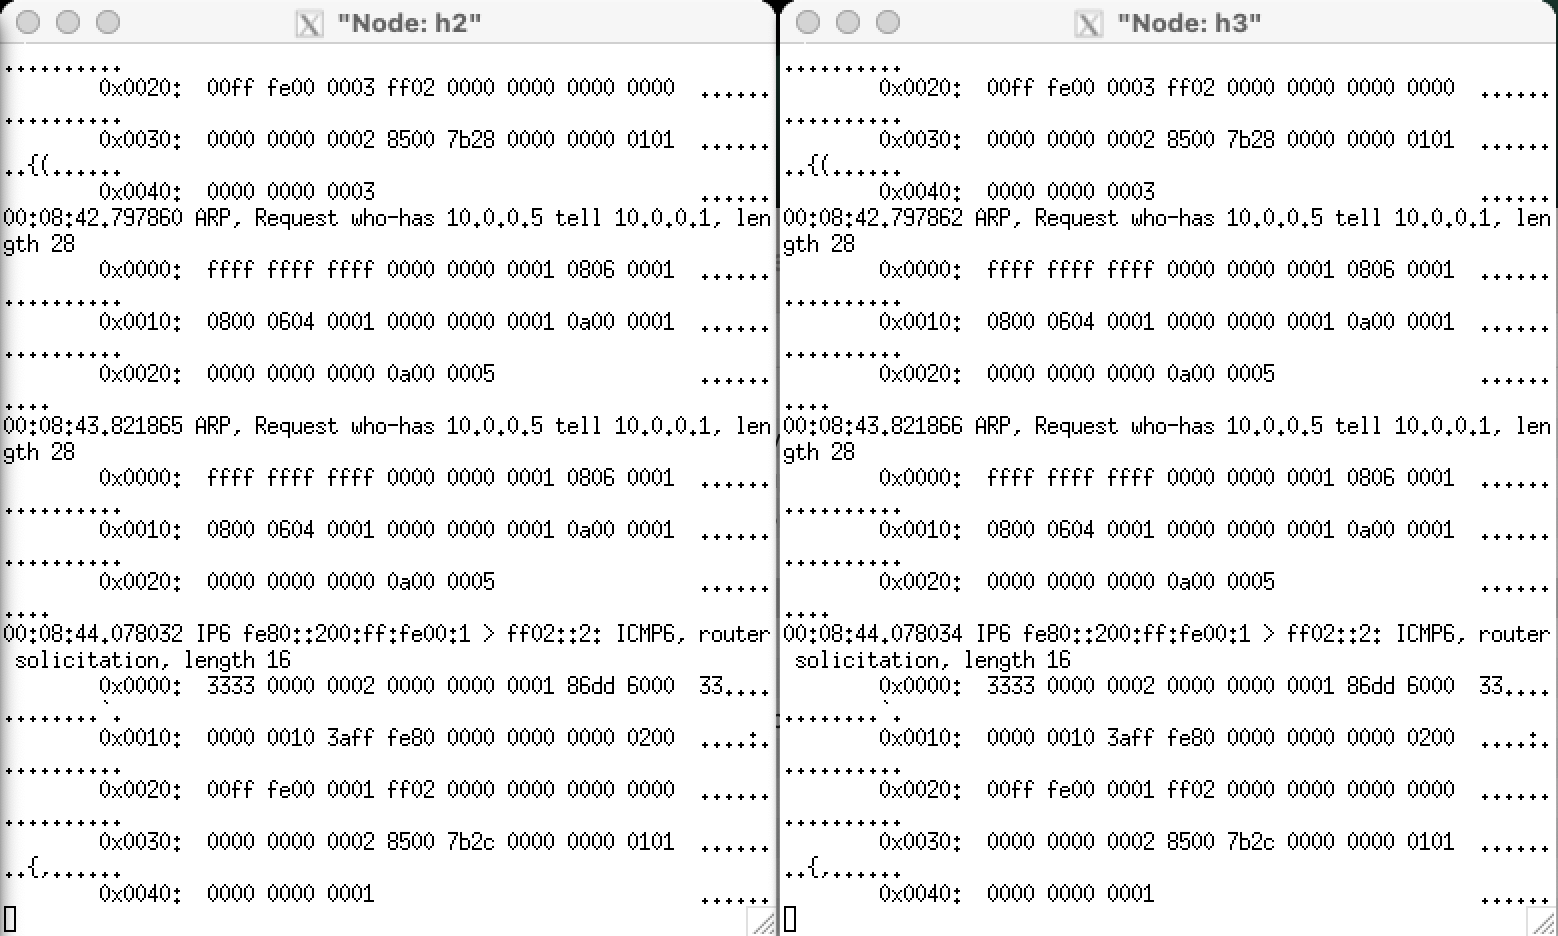
\includegraphics[width=\textwidth]{images/arp-non-exists.png}
  \caption{Вывод tcpdump после второго запроса ping}
  \label{fig:arp-non-exists}
\end{figure}

\section*{Заключение}

\textbf{Вывод}: в данной лабораторной работой я научился работать с mininet,
создавать скрипты, моделирующие различные сетевые топологии, а также тестировать
доступность различных хостов.

\newpage

\appendix

\titleformat{\section}[display]
{\normalfont\bfseries}
{\centering Приложение\ \thesection}
{0pt}{\centering}
\renewcommand{\thesection}{\Asbuk{section}}

\section{Исходный код скрипта линейной топологии}
\label{app:LinearTopo.py}

\begin{code}
  \inputminted{python}{../code/LinearTopo.py}
\end{code}

\newpage

\section{Исходный код скрипта древовидной топологии}
\label{app:CustomTopo.py}

\begin{code}
  \inputminted{python}{../code/CustomTopo.py}
\end{code}

\end{document}